\documentclass[a4paper, 12pt]{article}

% Better font selection
\usepackage{fontspec}

% PDF hyperlinks
\usepackage{hyperref}

% Graphics
\usepackage{tikz}
\usetikzlibrary{positioning}

% Unicode math symbols
\usepackage{unicode-math}
% Use a math font which has support for "\"
\setmathfont{Libertinus Math}

% Mathematical commands
\usepackage{amsmath}
\usepackage{amsthm}
\usepackage{mathtools}

% Set notation
\usepackage{braket}

% Support for commenting out blocks of LaTeX code
\usepackage{verbatim}

\theoremstyle{definition}
\newtheorem*{theorem}{Theorem}
\newtheorem*{corollary}{Corollary}
\newtheorem*{definition}{Definition}

\newcommand{\naturals}{\symbb{N}}
\newcommand{\reals}{\symbb{R}}
\newcommand{\complex}{\symbb{C}}
\newcommand{\ball}{\symcal{B}}

\DeclarePairedDelimiter{\ceil}{\lceil}{\rceil}
\DeclarePairedDelimiter{\norm}{\lVert}{\rVert}

% Command to number only one line in a multi-line equation
% Based on https://tex.stackexchange.com/a/42728
\newcommand\numberthis{\addtocounter{equation}{1}\tag{\theequation}}

\title{Proof of the open mapping theorem}
\author{Gabriel Majeri}
\date{}

\begin{document}

\maketitle

\begin{theorem}[Open mapping]
Let \(X\) and \(Y\) be two \textbf{complete metric spaces} and \(\Lambda \colon X \to Y\) a \textbf{surjective} and \textbf{bounded} \textbf{linear transformation} between them. Denote with \(U \subset X\) and \(V \subset Y\) the corresponding open unit balls. Then there exists a \(\delta > 0\) such that
\[
    \Lambda(U) \supseteq \delta V
\]
where \(\delta V = \Set{ \delta \cdot v \mid v \in V }\) is the open ball of radius \(\delta\) centered at \(0 \in Y\).
\end{theorem}

This is a graphical representation of the statement of the theorem:
\begin{figure}[h!]
    \centering
        
    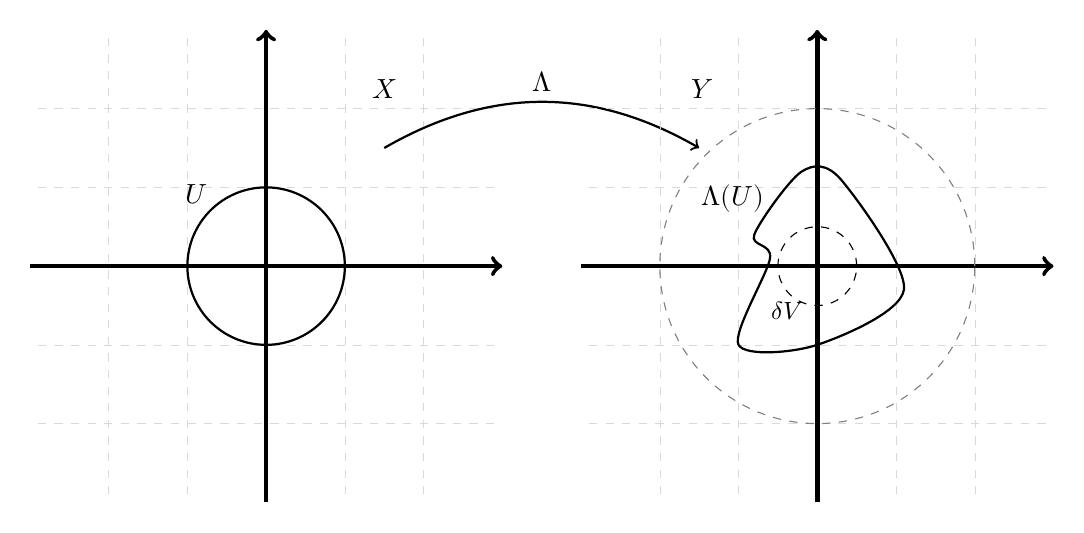
\begin{tikzpicture}
        \draw (1.5,2.25) node {\(X\)};
        \draw[help lines, color=gray!30, dashed] (-2.9,-2.9) grid (2.9,2.9);
        \draw[->,ultra thick] (-3,0)--(3,0);
        \draw[->,ultra thick] (0,-3)--(0,3);

        \draw[thick] (0,0) circle (1) node (U) {};
        \node[above left = 0.75 of U] {\(U\)};
        
        \draw[->, thick] (1.5, 1.5) to [out=30,in=150] node[above] {\(\Lambda\)} ++(4, 0);
        
        \begin{scope}[shift={(7, 0)}]
            \draw (-1.5,2.25) node {\(Y\)};
            \draw[help lines, color=gray!30, dashed] (-2.9,-2.9) grid (2.9,2.9);
            \draw[->,ultra thick] (-3,0)--(3,0);
            \draw[->,ultra thick] (0,-3)--(0,3);
            
            \draw [thick] node (LambdaU) {} plot [smooth cycle] coordinates {(-0.6,0.1) (-0.8,0.4) (-0.2,1.2) (0.3,1.1) (1.1,-0.3) (0,-1) (-1, -1)};
            \node[above left = 0.6 of LambdaU] {\(\Lambda(U)\)};

            \draw[dashed] (0,0) circle (0.5) node (DeltaV) {};
            \node[below left = 0.2 and 0 of DeltaV] {\small \(\delta V\)};
            \draw[dashed, gray] (0,0) circle (2);
        \end{scope}
    \end{tikzpicture}
\end{figure}

Since \(\Lambda\) is bounded, we are certain that \(\Lambda(U)\) is contained within some multiple of the open unit ball \(V\). What the theorem further shows is that, if the metric spaces are complete and \(\Lambda\) is surjective, we can also fit some multiple of the open unit ball \emph{within} \(\Lambda(U)\).

If we replace \(U\) in the hypothesis with some other open ball \(B\) of center \(c\), through linearity we get that \(\Lambda(B)\) contains an open neighborhood of \(\Lambda(c)\). Hence, \(\Lambda\) maps open sets to open sets, which makes it an open map. This is why the result is also known as the \textbf{open mapping theorem}.

\begin{proof}
First, we will show that we can fit an open ball within some multiple of the image of \(U\).

Let \(y \in Y\). Since \(\Lambda\) is surjective, there exists some \(x \in X\) such that \(\Lambda(x) = y\). Let \(k\) be the smallest integer such that \(k > \norm{x}\). Then \(x \in kU\) (the unit ball scaled by \(k\)), hence \(y \in \Lambda(kU)\). Since \(y\) was arbitrary, this shows that
\begin{equation} \label{decomposition_of_y}
    Y = \bigcup_{k = 1}^{\infty} \Lambda (kU)
\end{equation}

\begin{figure}[h!]
    \centering
    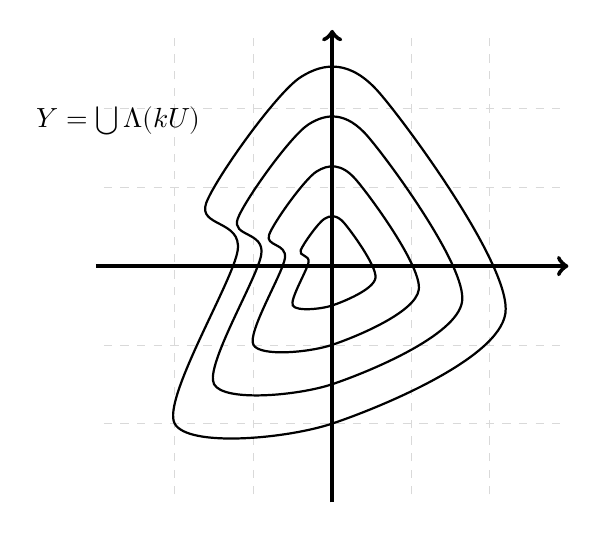
\begin{tikzpicture}
        \draw[help lines, color=gray!30, dashed] (-2.9,-2.9) grid (2.9,2.9);
        \draw[->,ultra thick] (-3,0)--(3,0);
        \draw[->,ultra thick] (0,-3)--(0,3);
        
        \draw [thick, scale=0.5] node (LambdaU) {} plot [smooth cycle] coordinates {(-0.6,0.1) (-0.8,0.4) (-0.2,1.2) (0.3,1.1) (1.1,-0.3) (0,-1) (-1, -1)};

        \draw [thick, scale=1] node (2LambdaU) {} plot [smooth cycle] coordinates {(-0.6,0.1) (-0.8,0.4) (-0.2,1.2) (0.3,1.1) (1.1,-0.3) (0,-1) (-1, -1)};

        \draw [thick, scale=1.5] node (3LambdaU) {} plot [smooth cycle] coordinates {(-0.6,0.1) (-0.8,0.4) (-0.2,1.2) (0.3,1.1) (1.1,-0.3) (0,-1) (-1, -1)};
        
        \draw [thick, scale=2] node (4LambdaU) {} plot [smooth cycle] coordinates {(-0.6,0.1) (-0.8,0.4) (-0.2,1.2) (0.3,1.1) (1.1,-0.3) (0,-1) (-1, -1)};
        
        \node[above left = 2 of 4LambdaU] {\(Y = \bigcup \Lambda(kU)\)};
    \end{tikzpicture}
\end{figure}

Now, we will need to use another result known as the Baire category theorem.
\begin{theorem}[Baire]
If a complete metric space \(X\) is written as the union of a countable family of closed sets, then at least one of them has a non-empty interior.
\end{theorem}

By taking into consideration that \(Y\) is complete, and computing the closure for \ref{decomposition_of_y}, we obtain that there is at least one \(k'\) such that
\[
    \mathring{\overline{\Lambda(k' U)}} \neq \emptyset
\]
Therefore, there exists at least one open set \(V\) such that \(V \subset \overline{\Lambda(k'U)}\). Being open in a metric space means that we can fit an open ball \(\ball_r (c)\) inside \(V\), with radius \(r \in \reals^*_+\) and center \(c \in V\).
\begin{figure}[!ht]
    \centering
    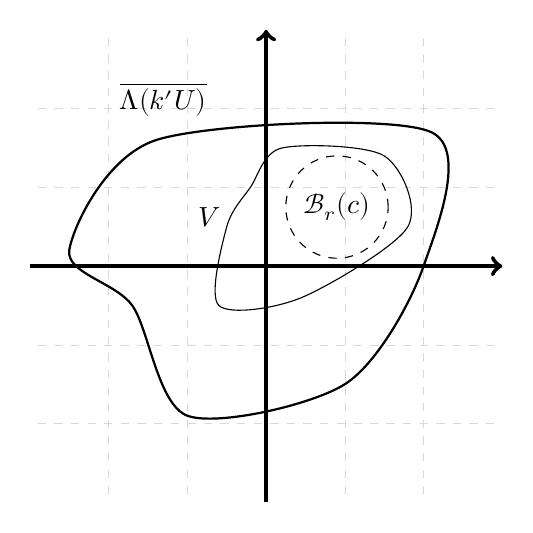
\begin{tikzpicture}
        \draw[help lines, color=gray!30, dashed] (-2.9,-2.9) grid (2.9,2.9);
        \draw[->,ultra thick] (-3,0)--(3,0);
        \draw[->,ultra thick] (0,-3)--(0,3);
        
        \draw [thick] node (LambdaKPrimeU) {} plot [smooth cycle] coordinates {(-2.5, 0.2) (-1.4,1.6) (2.1,1.7) (2,0) (1,-1.5) (-1,-1.9) (-1.7, -0.5)};
        \node[above left = 1.65 and 0.5 of LambdaKPrimeU] {\(\overline{\Lambda(k'U)}\)};
        
        \draw node (V) {} plot [smooth cycle] coordinates {(-0.2, 1) (0.2, 1.5) (1.5, 1.4) (1.8, 0.5) (0.45, -0.4) (-0.6, -0.5) (-0.5, 0.5)};
        \node[above left = 0.25 and 0.4 of V] {\(V\)};

        \draw[dashed] (0.9,0.75) circle (0.65) node {\(\ball_r(c)\)};
    \end{tikzpicture}
\end{figure}

Let \(y \in Y\) be a vector with \(\norm{y} < r\). Then:
\begin{gather*}
    \norm{y} < r \\
    \implies \norm{c - c + y} < r \\
    \implies d(c, c + y) < r \\
    \implies c + y \in \ball_r (c)
\end{gather*}

Since \(c \in V \subset \overline{\Lambda(k'U)}\) and \(c + y \in \ball_r (c) \subset V \subset \overline{\Lambda(k'U)}\), by the definition of the closure of a set we can find sequences \((y'_n)_{n \in \naturals} \subset \Lambda(k'U)\) and \((y''_n)_{n \in \naturals} \subset \Lambda(k'U)\) such that
\begin{align*}
    y'_n &\rightarrow c \\
    y''_n &\rightarrow c + y
\end{align*}

By the continuity of \(\Lambda\), there exist two corresponding sequences \((x'_n)_{n \in \naturals} \subset k'U\), \((x''_n)_{n \in \naturals} \subset k'U\) such that
\begin{align*}
    \Lambda(x'_n) &= y'_n \\
    \Lambda(x''_n) &= y''_n
\end{align*}

Denote \(x_n = x''_n - x'_n\). By the linearity of \(\Lambda\) we have that
\begin{gather*}
    \Lambda(x_n) = \Lambda(x''_n - x'_n) = \Lambda(x''_n) - \Lambda(x'_n) = y''_n - y'_n
\end{gather*}
The difference of two convergent sequences converges to the limit of the differences, so
\begin{equation} \label{limit_of_lambda_xn}
    \lim_{n \to \infty} \Lambda(x_n) = \lim_{n \to \infty} \left(y''_n - y'_n\right) = y
\end{equation}

The distance between any two points \(x'_n\) and \(x''_n\) of the open ball \(k'U = \ball_{k'} (0)\) is at most its diameter, therefore
\begin{equation} \label{norm_of_xn}
    \norm{x_n} = \norm{x''_n - x'_n} < 2k'
\end{equation}

Using linearity, we can scale \ref{limit_of_lambda_xn} and \ref{norm_of_xn} by \(\norm{y}/r > 0\). Denoting with \(\widetilde{x}_n = \frac{\norm{y}}{r} x_n\), we obtain
\[
    \lim_{n\to\infty} \Lambda(\widetilde{x}_n) = y \frac{\norm{y}}{r}
\]
and
\[
    \norm{\widetilde{x}_n} < \frac{2k'}{r} \norm{y}
\]
We will denote the quantity \(\frac{r}{2k'}\) by \(\delta\). Thus, the last inequality can be restated as
\[
    \norm{\widetilde{x}_n} < \delta^{-1} \norm{y}
\]

Linearity also allows us to expand the above results to all of \(Y\). If \(\norm{y'} \geq r\), then we can find a \(y\) with \(\norm{y} < r\) such that \(y' = \lambda y\) for some \(\lambda > 0\). Define \(\widetilde{x}'_n = \lambda \widetilde{x}_n\), and the statements still hold.

Rewriting \ref{limit_of_lambda_xn} using the definition of the limit and combining it with \ref{norm_of_xn}, we obtain that \(\forall y \in Y\) and \(\forall \epsilon > 0\), there exists an \(x \in X\) with
\begin{equation} \label{definition_of_x}
    \norm{x} < \delta^{-1} \norm{y} \text{ and } \norm{y - \Lambda(x)} < \epsilon
\end{equation}
(we can simply take \(x = x_{N_\epsilon}\)).

Now we are ready to prove the theorem. Let \(y \in \delta V\) and fix some \(\eta > 0\). We apply \ref{definition_of_x} with \(\epsilon = \frac{1}{2} \delta \eta\) and obtain an \(x_0\) with the properties
\[
    \norm{x_0} < \delta^{-1} \norm{y} = \delta^{-1} \delta = 1
\]
and
\[
    \norm{y - \Lambda(x_0)} < \frac{1}{2} \delta \eta
\]

We can proceed inductively. Suppose we have \(x_0, x_1, \dots, x_n\). We apply \ref{definition_of_x} to \(y - \Lambda(x_0) - \Lambda(x_1) - \dots - \Lambda(x_n)\) with \(\epsilon = \frac{1}{2^{n + 1}} \delta\) and we obtain an \(x_{n + 1}\) with
\[
    \norm{x_{n + 1}} < \delta^{-1} \norm{y - \Lambda(x_0) - \Lambda(x_1) - \dots - \Lambda(x_n) } < \delta^{-1} \frac{1}{2^{n + 1}} \delta \eta = \frac{1}{2^{n + 1}} \eta
\]
and
\begin{equation} \label{xn_inequality}
    \norm{y - \Lambda(x_1) - \Lambda(x_2) - \dots - \Lambda(x_{n + 1})} < \frac{1}{2^{n + 1}} \delta \eta
\end{equation}
From this, we conclude that \(\norm{x_n} < \frac{1}{2^n} \eta\), \(\forall n \in \naturals^*\).

Now consider the sequence \((\overline{x_n}) \subset X\), where
\[
    \overline{x_n} = \sum_{i = 1}^{n} x_i
\]
We remark that \(\norm{\overline{x_n} - \overline{x_{n - 1}}} = \norm{x_n} < \frac{1}{2^n} \eta, \forall n \in \naturals^*\), therefore the sequence is Cauchy. Because \(X\) is complete, it means \((\overline{x_n})\) is convergent to some point \(\overline{x} \in X\). Using the triangle inequality, we get that
\begin{equation} \label{bound_on_x_bar}
    \norm{\overline{x}} = \norm*{\sum_{i=0}^{\infty} x_i}
    \leq \sum_{i=0}^{\infty} \norm*{x_i} < \sum_{i=0}^{\infty} \frac{1}{2^i} \eta = 1 + \eta
\end{equation}

Since \(\Lambda\) is linear, the inequality \ref{xn_inequality} can be rewritten as
\begin{align*}
    \norm{y - \Lambda(x_1 + \dots + x_{n+1})} &< \frac{1}{2^{n+1}} \delta \eta \iff \\
    \norm{y - \Lambda(\overline{x_{n+1}})} &< \frac{1}{2^{n+1}} \delta \eta
\end{align*}
We take the limit of this inequality:
\[
    \lim_{n\to\infty} \norm{y - \Lambda(\overline{x_{n+1}})} = 0
\]
and use the continuity of the norm and of \(\Lambda\) to conclude that \(y = \Lambda(\overline{x})\). Therefore, \(y \in (1 + \eta) \, U\). We took \(y \in \delta V\), so
\[
    \delta V \subseteq \Lambda((1 + \eta) \, U)
\]
We can rewrite this using linearity as
\[
    \frac{1}{1 + \eta} \, \delta V \subseteq \Lambda(U)
\]
for all \(\eta > 0\). By taking the union of all \(\frac{1}{1 + \eta} \delta V\) we obtain \(\delta V\), which shows that
\[
    \delta V \subseteq \Lambda(U)
\]
\end{proof}

We will now prove an immediate consequence of the open mapping theorem:
\begin{theorem}[Bounded inverse]
Let \(X\) and \(Y\) be two \textbf{complete metric spaces} and \(\Lambda \colon X \to Y\) a \textbf{bijective} and \textbf{bounded} \textbf{linear transformation} between them. Then \(\Lambda^{-1}\) is also a \textbf{bounded} \textbf{linear transformation}.
\end{theorem}
\begin{proof}
Since \(\Lambda\) is bijective, we know that the inverse \(\Lambda^{-1} \colon Y \to X\) exists. Furthermore, we know it is a linear transformation.

\begin{comment}
Furthermore, we can check that it is a linear transformation. We know \(\Lambda\) is linear, therefore
\[
    a \Lambda(u) + b \Lambda(v) = \Lambda(au + bv)
\]
for all \(a, b \in \complex\), \(u, v \in X\). Then, by applying \(\Lambda^{-1}\) to the equation we get
\[
    \Lambda^{-1} (a \Lambda(u) + b \Lambda(v)) = \Lambda^{-1}(\Lambda(au + bv)) = au + bv
\]
If we denote \(\Lambda(u)\) with \(u'\), \(\Lambda(v)\) with \(v'\), then \(u = \Lambda^{-1}(u')\) and \(v = \Lambda^{-1}(v')\). We have that
\[
    \Lambda^{-1} (a u' + b v') = a \Lambda^{-1} (u') + b \Lambda^{-1} (v')
\]
for all \(u', v' \in Y\), since \(\Lambda\) is surjective.
\end{comment}

To prove that it is also bounded, by definition we need to show that there exists a \(\delta' > 0\) such that
\[
    \norm{\Lambda^{-1}(y)} \leq \delta' \norm{y}, \forall y \in Y
\]
Since \(\Lambda\) is bijective, by letting \(y = \Lambda(x)\) we obtain the equivalent statement:
\[
    \norm{x} \leq \delta' \norm{\Lambda(x)}, \forall x \in X
\]
Moving \(\delta'\) to the left, we get:
\[
    \delta'^{-1} \norm{x} \leq \norm{\Lambda(x)}, \forall x \in X
\]

Let \(\delta > 0\) be the constant we get for this hypothesis from the open mapping theorem. We know that every \(y \in Y\) with \(\norm{y} < \delta\) is the image \(\Lambda(x)\) of some \(x \in X\) with \(\norm{x} < 1\). But since \(\Lambda\) is bijective, this \(x\) is unique; there cannot be another \(x'\) (with norm possibly greater than \(1\)) such that \(\Lambda(x') = y\). So \(\norm{\Lambda(x)} < \delta \implies \norm{x} < 1\).

By negating this proposition, we obtain that when \(\norm{x} \geq 1\) we must have \(\norm{\Lambda(x)} \geq \delta\).

Setting \(\delta'^{-1} = \delta\), the condition above can be rewritten as:
\[
    \norm{\Lambda(x)} \geq \delta \norm{x}, \forall x \in X
\]
which is true based on the linearity of \(\Lambda\).
\end{proof}
\end{document}
